\section{Blockchain}

\subsection{Cos'è?}
Una blockchain è una struttura pubblica, condivisa e immutabile che permette di
salvare dati all'interno di blocchi. I blocchi sono collegati tra loro in modo
tale che ogni blocco verifichi il successivo e per questo modo se un nodo della
catena si rompe, allora tutta la catena viene invalidata.

\subsection{Parole chiave}
Si usa parola \textbf{blocco} per indicare un insieme di informazioni che
vengono salvate all'interno della blockchain. Infatti i dati non sono inseriti
singolarmente come in un database tradizionale, ma vengono raggruppati in
blocchi di dimensione predefinita e una volta che viene soddisfatta la
dimensione vengono salvati.

Una \textbf{catena} è l'insieme dei blocchi collegati tra loro. Ogni blocco è 
collegato al blocco precedente tramite un codice hash creando in questo modo
un legame inviolabile, dato che la modifica di un blocco porterebbe al 
cambiamento del codice hash e quindi all'invalidazione di tutti i collegamenti
successivi.

Un \textbf{hash code} è un codice che viene generato da una funzione matematica
che a partire da una stringa di lunghezza variabile, ne genera una di lunghezza
fissa che identifica univocamente la stringa di partenza. Può essere visto come
se fosse l'impronta digitale dell'elemento di partenza in quanto è unica e 
rappresenta in modo diretto l'input iniziale. Il codice hash risulta differente
anche se un solo carattere della stringa di partenza viene modificato, quindi è 
facile intuire che se un blocco cambia hash code, allora sicuramente è stato
mutato.

Ogni computer all'interno della rete blockchain è chiamato \textbf{nodo} e
si occupa di verificare che i blocchi siano validi e di aggiungerli alla
catena, in questo modo la catena non è presente su un solo computer, ma è 
\textbf{distribuita} su tutti i nodi della rete.

Le operazioni che vengono svolte all'interno di questa struttura sono chiamate
\textbf{transazioni} e sono salvate all'interno dei blocchi.

Ora che abbiamo definito le parole chiave della blockchain possiamo andare ad
analizzare in dettaglio il funzionamento di questa tecnologia.

\newpage

\subsection{Come funziona?}
La blockchain è per certi versi simile a un database, ossia il suo scopo è
salvare dati di vario tipo, ma ciò che li differenzia è il modo in cui i dati
vengono salvati. \\ 
Come detto prima la blockchain è una serie di blocchi che contengono
informazioni, in particolare vengono salvati tre dati:
\begin{itemize}
    \item \textbf{Dati}: sono i dati che devono essere salvati. La tipologia di 
        dati può variare in base al tipo di blockchain utilizzata.
    \item \textbf{Hash del blocco precedente}: è l'hash del blocco precedente
        e serve per collegare i blocchi tra loro. Se il blocco precedente viene
        modificato e il suo hash code  cambia, allora non sarà più uguale a
        quello salvato nel blocco successivo e quindi la catena viene
        invalidata.
    \item \textbf{Hash}: è un codice univoco che identifica il blocco e viene
        calcolato in base ai dati contenuti nel blocco stesso. Per poterlo
        calcolare si una appunto una funzione di hashing che prende in input
        i dati e restituisce l'hash.
\end{itemize}

\begin{figure}[H]
    \centering
    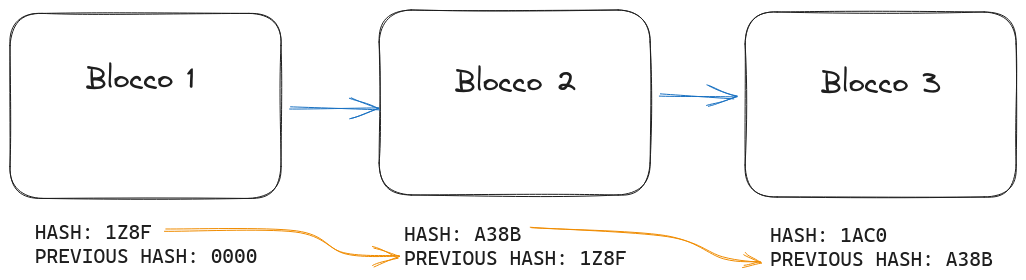
\includegraphics[width=0.9\textwidth]{BlocksSchema.png} 
    \caption{Schema dei blocchi Blockchain}
    \label{fig:chain}
\end{figure}

Dall'immagine precedente \ref{fig:chain} si può notare che ogni blocco
è collegato al blocco prima tramite l'hash del blocco precedente. 
Il primo blocco ha come hash precedente \textit{0000} perchè essendo il blocco
iniziale non esistono blocchi prima di lui.

\begin{figure}[H]
    \centering
    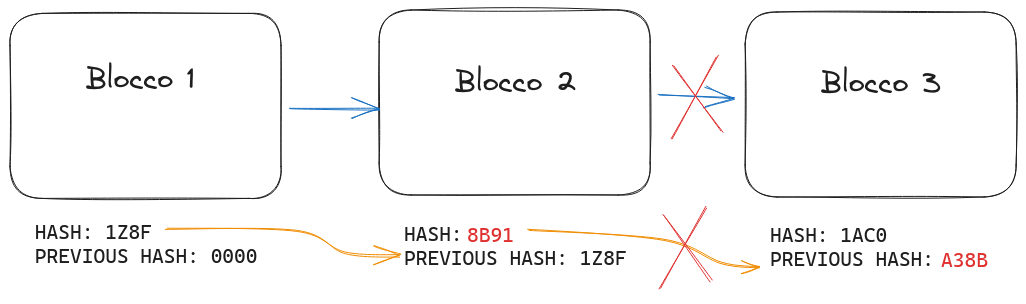
\includegraphics[width=0.9\textwidth]{BlocksSchemaInvalid.png} 
    \caption{Catena invalida}
    \label{fig:invalidChain}
\end{figure}

In questo caso \ref{fig:invalidChain} si può notare che il blocco 2 è stato
modificato e quindi il suo hash code è cambiato. Questo ha portato alla
invalidazione della catena in quanto il blocco 3 non ha più come hash del
blocco precedente quello del blocco 2.

